\documentclass{article}
\usepackage{graphicx}
\usepackage{float}

\begin{document}

\title{Assignment Scientific Visualization \\ \large{Stationary Fluid Mixer}}
\author{Paulo Liedtke \\ Student Number: 14209772}
\date{\today}

\maketitle

\section{Introduction}
In this Assignment I created a visualization of a stationary (static) fluid mixer. The data file is a .vtk file that contains the xxx of the fluid.
Those static mixers are used for the continuous mixing of fluid materials, without moving components. An example is the mixing of two-component adhesives, wastewater treatment or chemical processing.
The objective of this visualization is to answer the question if this mixer in fact mixes the fluids or if they are still separated after the process. 

\section{Approach}
I used ParaView to implement the visualization pipeline. The following steps describe the approach I used to create a visualization that is similar to the reference image.

\begin{enumerate}
    \item \textbf{Data Loading}: Imported the \texttt{SMRX.vtk} file into ParaView.
    
    \item \textbf{Outline Representation}: Modified the representation of \texttt{SMRX.vtk} to 'Outline', displaying a white box around the data
    
    \item \textbf{Contour Filter Application}: Applied a contour filter with the isosurfaces value set to 2 and changed the coloring to solid coloring (brown)
    
    \item \textbf{Streamtracer Addition}: Added two streamtracers to illustrate the fluid flow
    
    \item \textbf{Seed Type Configuration and different Y Values}: Configured the seed type of both streamtracers to 'Line', with endpoints within the outlined box. The first streamtracer's endpoints were set to (0.1, 40, 0.1) and (0.1, 40, 59), while the second streamtracer's endpoints were set to (0.1, 20, 0.1) and (0.1, 20, 59) resulting into different y values.
        
    \item \textbf{Integration Direction Setting}: Set the integration direction for both streamtracers to 'Forward'.
    
    \item \textbf{Color Adjustment}: Changed the streamline colors to green and blue for each streamtracer, respectively.
    
    \item \textbf{Streamline Length Modification}: Increased the maximum streamline length to 150 to ensure streamlines reach end of the Outline.
    
    \item \textbf{Resolution Reduction}: Reduced the resolution to 100 to make the visualization more close to the reference image.
\end{enumerate}

I used the default capture screenshot feature of ParaView to save the visualization as a .png file. 

\section{Results}

The figures \ref{fig:top-view} and \ref{fig:side-view} show a top and side view of the mixer.

\begin{figure}[H]
    \centering
    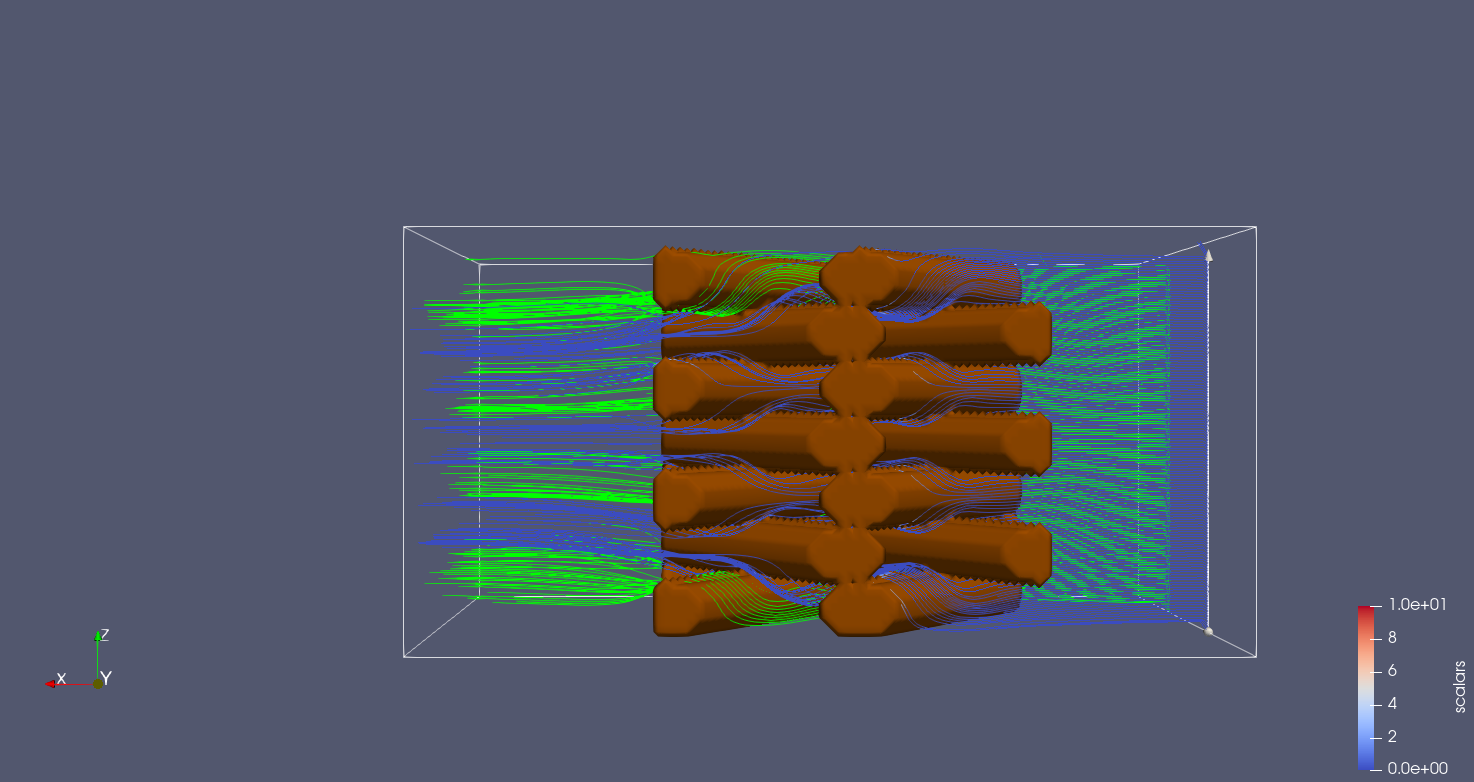
\includegraphics[width=0.8\textwidth]{top-view.png}
    \caption{Top View}
    \label{fig:top-view}
\end{figure}

\begin{figure}[H]
    \centering
    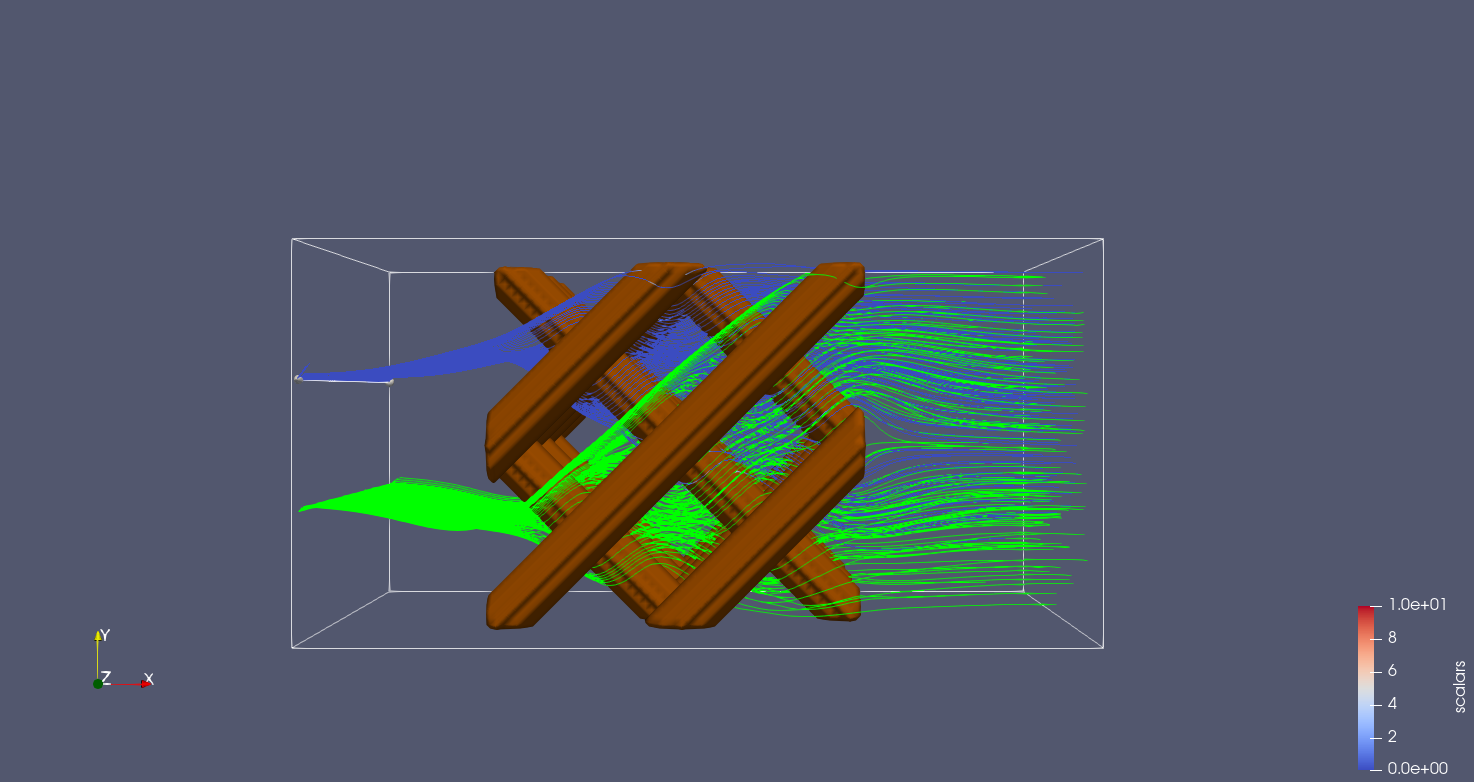
\includegraphics[width=0.8\textwidth]{side-view.png}
    \caption{Side View}
    \label{fig:side-view}
\end{figure}

Figure \ref{fig:reference} shows the reference image of the static mixer. Figure \ref{fig:static_mixer} shows a viery similar image of the visualization pipeline that I built.


\begin{figure}[H]
    \centering
    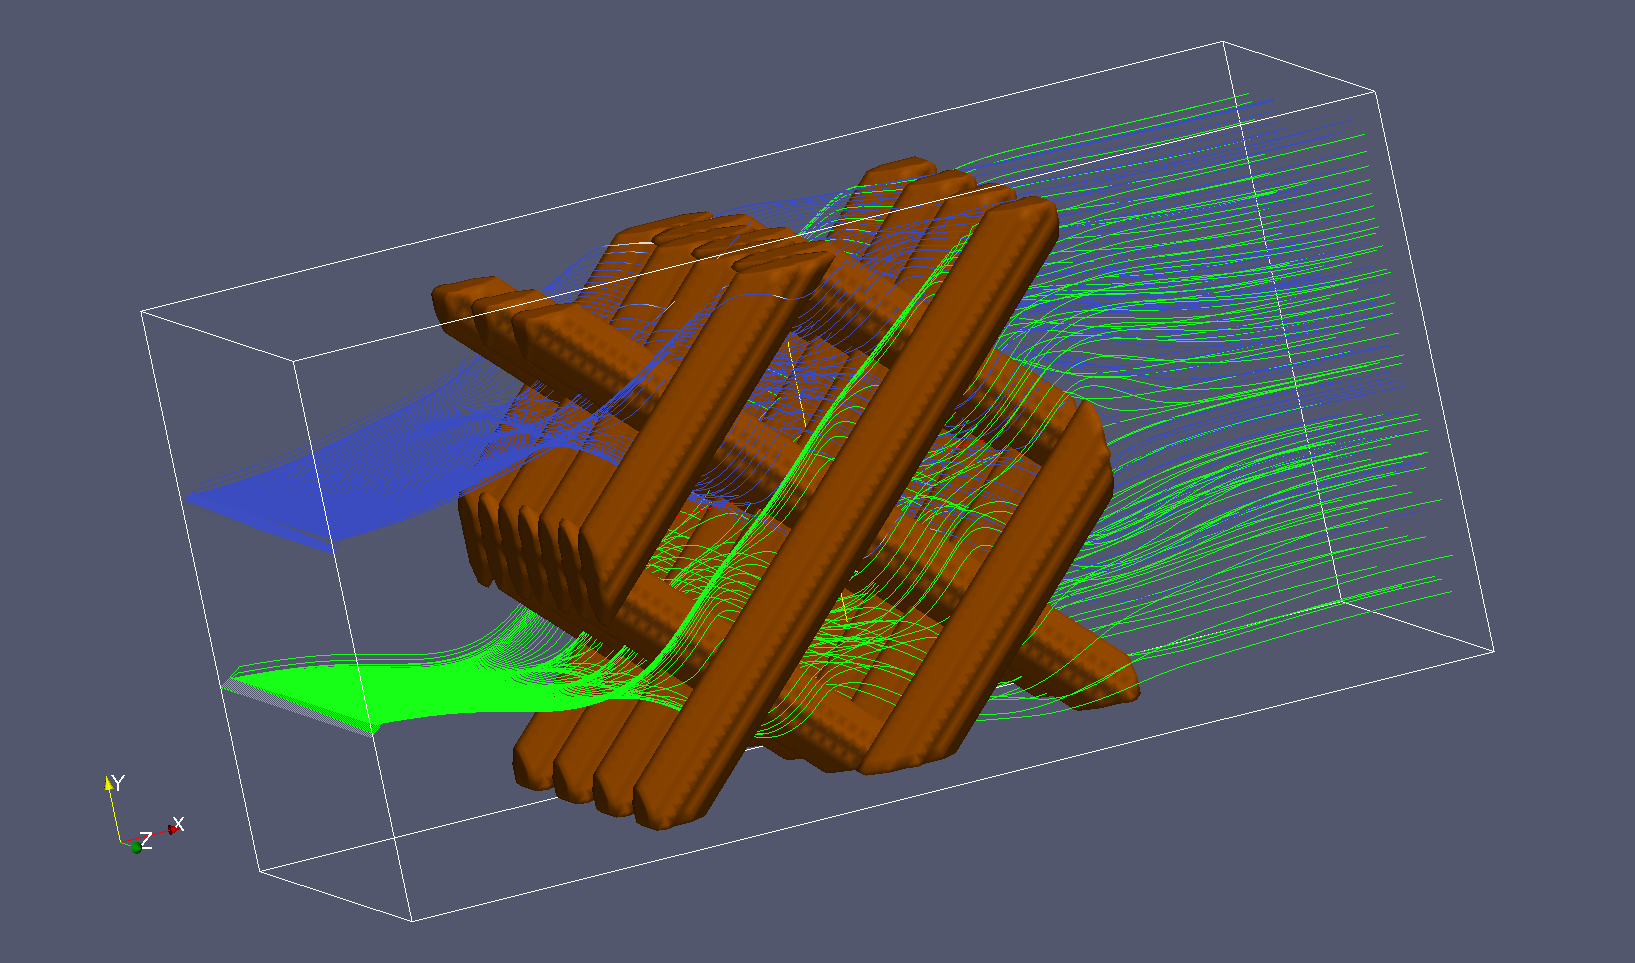
\includegraphics[width=0.8\textwidth]{reference.png}
    \caption{Reference Image}
    \label{fig:reference}
\end{figure}

\begin{figure}[H]
    \centering
    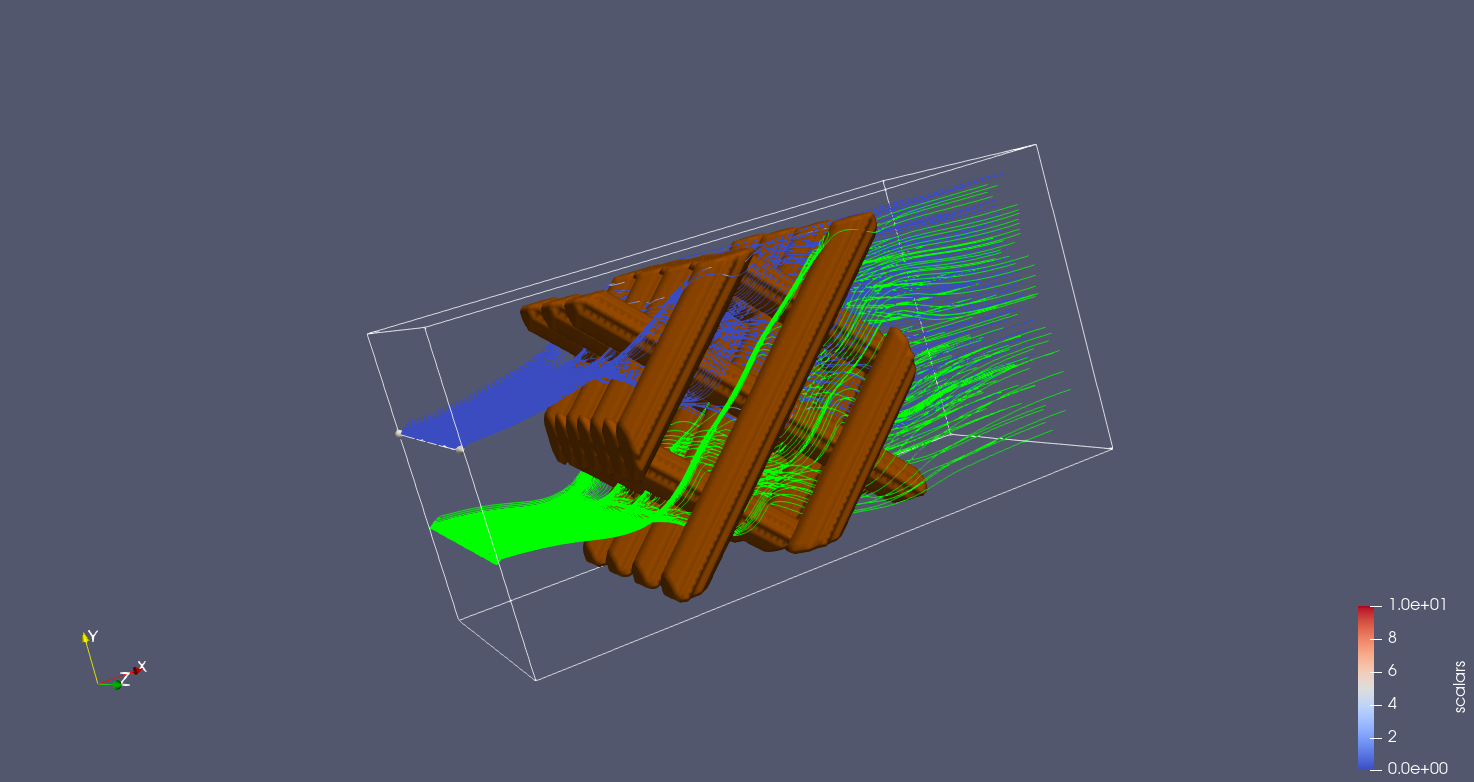
\includegraphics[width=0.8\textwidth]{final.png}
    \caption{Static Mixer}
    \label{fig:static_mixer}
\end{figure}

\section{Discussion}
From the figure \ref{fig:top-view} can be seen that fluids from the StreamTracer follow the structure of the mixer.
From the side view \ref{fig:side-view} it can be seen that the fluids are indeed getting mixed.

\end{document}0